%! TEX root = ../../master.tex
\lecture[Template cuts and examples for $\TSP$. Knapsack cover for binary variables. Facet-inducing cuts.]{Th 30 June 2022}{Special CP techniques}

\begin{definition}
    \vocab{Template cuts}.
\end{definition}
For $\TSP$ we consider 2-matching CPs.
We know there is a polynomial algorithm for $\SEP$ of 2-matching CPs.\todo{ref script}
For subtour elimination cuts there also exists a polynomial $\SEP$-algorithm via MaxFlow/MinCut.
\vspace{5pt}
\\
\begin{minipage}{\textwidth}
    \centering
    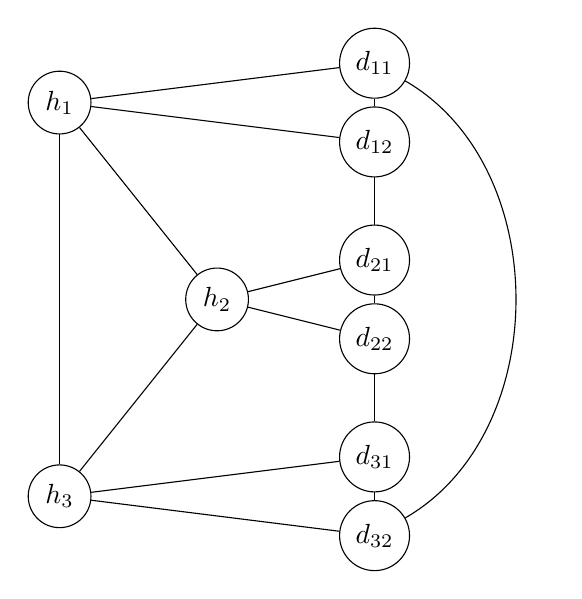
\begin{tikzpicture}
        \begin{scope}[every node/.style={draw, circle}]

            \node (h1) at (0,5) {$h_1$};
            \node (h2) at (2,2.5) {$h_2$};
            \node (h3) at (0,0) {$h_3$};

            \node (d11) at (4,5.5) {$d_{11}$};
            \node (d12) at (4,4.5) {$d_{12}$};
            \node (d21) at (4,3) {$d_{21}$};
            \node (d22) at (4,2) {$d_{22}$};
            \node (d31) at (4,0.5) {$d_{31}$};
            \node (d32) at (4,-0.5){$d_{32}$};

        \end{scope}
        \path (h1) edge (h2);
        \path (h2) edge (h3);
        \path (h3) edge (h1);

        \path (h1) edge (d11);
        \path (h1) edge (d12);
        \path (h2) edge (d21);
        \path (h2) edge (d22);
        \path (h3) edge (d31);
        \path (h3) edge (d32);

        \path (d11) edge (d12);
        \path (d12) edge (d21);
        \path (d21) edge (d22);
        \path (d22) edge (d31);
        \path (d31) edge (d32);

        \path (d11) edge[bend left=60] (d32);
    \end{tikzpicture}
    % \captionof{figure}{A graph with $S$ colored orange}
\end{minipage}
\begin{lemma}
    This $x$ satisfies all degree, subtour, and 2-matching constraints.
\end{lemma}
\begin{proof}
    Brute Force.
\end{proof}
\todo{define comb}
\begin{theorem}[Chv\'atal]
    Let $T_1, \dots, T_k$ be mutually disjoint for odd $k$ such that
    $T_j \cap H \neq \emptyset$ and $T_j \cap H \setminus \emptyset$ for all $j$.
    Then
    \begin{align*}
        x(E(H))+ \sum_jx(E(T_j))\leq |H|+\sum_j(|T_j|-1) - \left\lceil \frac{k}{2} \right\rceil
    \end{align*}
    is valid for the $\TSP$ integer hull.
\end{theorem}
\begin{proof}
    Using degree and subtour constraints for a $\CG$-proof. See homework \todo{insert ref}
\end{proof}
\begin{remark}
    It is not known if $\SEP$ for combs is $\pP$ or $\NPC$.
    Nonetheless, for special cases polynomial $\SEP$-algorithms are known.
    One can also use Gomory-Hu-Trees for a heuristic comb-$\SEP$.
\end{remark}
While $\TSP$-cuts are specifically good for $\TSP$, in general they might not be good at all.
Therefore, we need to find general templates for $\MIP$/$\IP$ that most of the times work satisfactory.

Lots of $\IP$s have $0-1$-decision variables.

Suppose $x \in \bool^n$ and a constraint $a^Tx \leq b$.
If $a_j < 0$, replace
\begin{enumerate}
    \item $x_j$ by $1-x_j$,
    \item $a_j$ by $-a_j > 0$, and
    \item $b$ by $b-a_j > 0$.
\end{enumerate}
So, assume w.l.o.g.\ $a_j \geq 0$ and $a_j \leq b$. We define $N = \{1,\dots, n\}$.
Consider $C \subseteq N$ such that $a(C)>b$.
Then, if $x_j=1$ for all $j \in C$, the solution is infeasible.
\begin{theorem}
    As a consequence, $x(C) \leq |C|-1$ is valid for the integer hull.
\end{theorem}
\begin{proof}
    Via Chv\'atal derivation, see \todo{homework}.
\end{proof}
\begin{definition}
    Such things we call a \vocab{Knapsack cover}.
    Furthermore,  a cover $C$ is \vocab{minimal} if for all $j \in C$ it holds that $C-j$ is \emph{not} a cover.
\end{definition}
Can we separate $x^0$ from Knapsack covers, that is decide if
\begin{align*}
    x^0(C) \leq |C|-1
\end{align*}
for all minimal covers $C$?
Note
\begin{align*}
    (1-x^0)(C) = \sum_{j \in C}(1-x^0_j)= |C|-x^0(C),
\end{align*}
therefore
\begin{align*}
                    &  & x^0(C)                  & \leq |C|-1            \\
    \Leftrightarrow &  & (1-x^0)(C) = |C|-x^0(C) & \geq |C| - (|C|-1)=1,
\end{align*}
so deciding
\begin{align*}
    1 \geq \min_{\text{cover }C}(1-x^0)(C)
\end{align*}
suffices if $x^0$ satisfies all Knapsack covers.
Unfortunately, this is $\NP$-hard, but in practice we can use Dynamic Programming, see \todo{homework}.

\begin{observe}
    It seems to be ideal to find CPs that are \vocab{facet-inducing} on $P^I$, i.e. the intersection with
    $P^I$ is a facet of it. Knowing $\dim(P^I)$ is therefore necessary.
\end{observe}
$\TSP$ itself is not full-dimensional because of its degree equality-constraints.
\begin{theorem}
    The integer hull for knapsack cover \emph{is} full-dimensional (if $a_j \leq b$).
\end{theorem}
\begin{proof}
    Note $0 \in P^I$. Furthermore, for all $j$ it holds that $a_j \leq b$ implies the unit vector $e^j \in P^I$.
    So we have $n+1$ affinely independent points, immediately leading to $P^I$ being full-dimensional.
\end{proof}
Now, consider $P^I$ is full-dimensional.
There exists several methods of proving if a CP $\alpha^Tx \leq \beta$ is facet-inducing:
\begin{enumerate}
    \item Find $\bar x$ such that $\alpha^T\bar x > \beta$, but $\bar x$ satisfies all constraint of $P^I$.
          However, we don't know all constraints of $P^I$.
    \item Find feasible, affinely independent $v^1,\dots,v^n \in P^I$ such that for all $i$ it holds $\alpha^Tv^i = \beta$
    \item If $c^Tx \leq d$ is some other valid constraint for $P^I$ with
          \begin{align*}
              P^I \cap \{\alpha^Tx \leq \beta\} = P^I \cap \{c^Tx \leq d\},
          \end{align*}
          then $(c,d)$ is a scalar multiple of $(\alpha,\beta)$.
\end{enumerate}